\subsection{Installationsanleitung}
Die folgenden Schritte führen Sie durch die Installation der - auf Android Studio basierenden - Entwicklungsumgebung. Diese ist für den Unterhalt und die Weiterentwicklung der TravelBuddy Mobile App erforderlich.

\subsubsection{Vorraussetzungen}
Für die erfolgreiche Installation ihrer Entwicklungsumgebung müssen folgende Gegebenheiten erfüllt sein:
\begin{enumerate}
  \item Die Virtualisierung muss im BIOS aktiviert sein, wie Sie diese aktivieren finden Sie im Handbuch der Hauptplatine ihres Rechners.
  \item Eine funktionierende Installation von git.exe
  \item Ihnen ist die grundlegende Arbeitsweise von Git bekannt und Sie wissen wie Sie ein Projekt von github.com klonen, synchronisieren und ihre Ergebnisse veröffentlichen.
  \item Sie wissen wie Sie die ``Git Bash'' Konsole starten und wie Sie sie verwenden.
  \item Sie verfügen über Administratoren Privilegien auf dem Zielrechner
\end{enumerate}

\subsubsection{Das Github Projekt}
Um eine möglichst gute Kollaboration zu ermöglichen wird beim Projekt TravelBuddy auf Git gesetzt.
Sie finden das Projekt unter: https://github.com/PsitTeam3/TravelBuddyAndroidApp
\begin{figure}
  \centering
  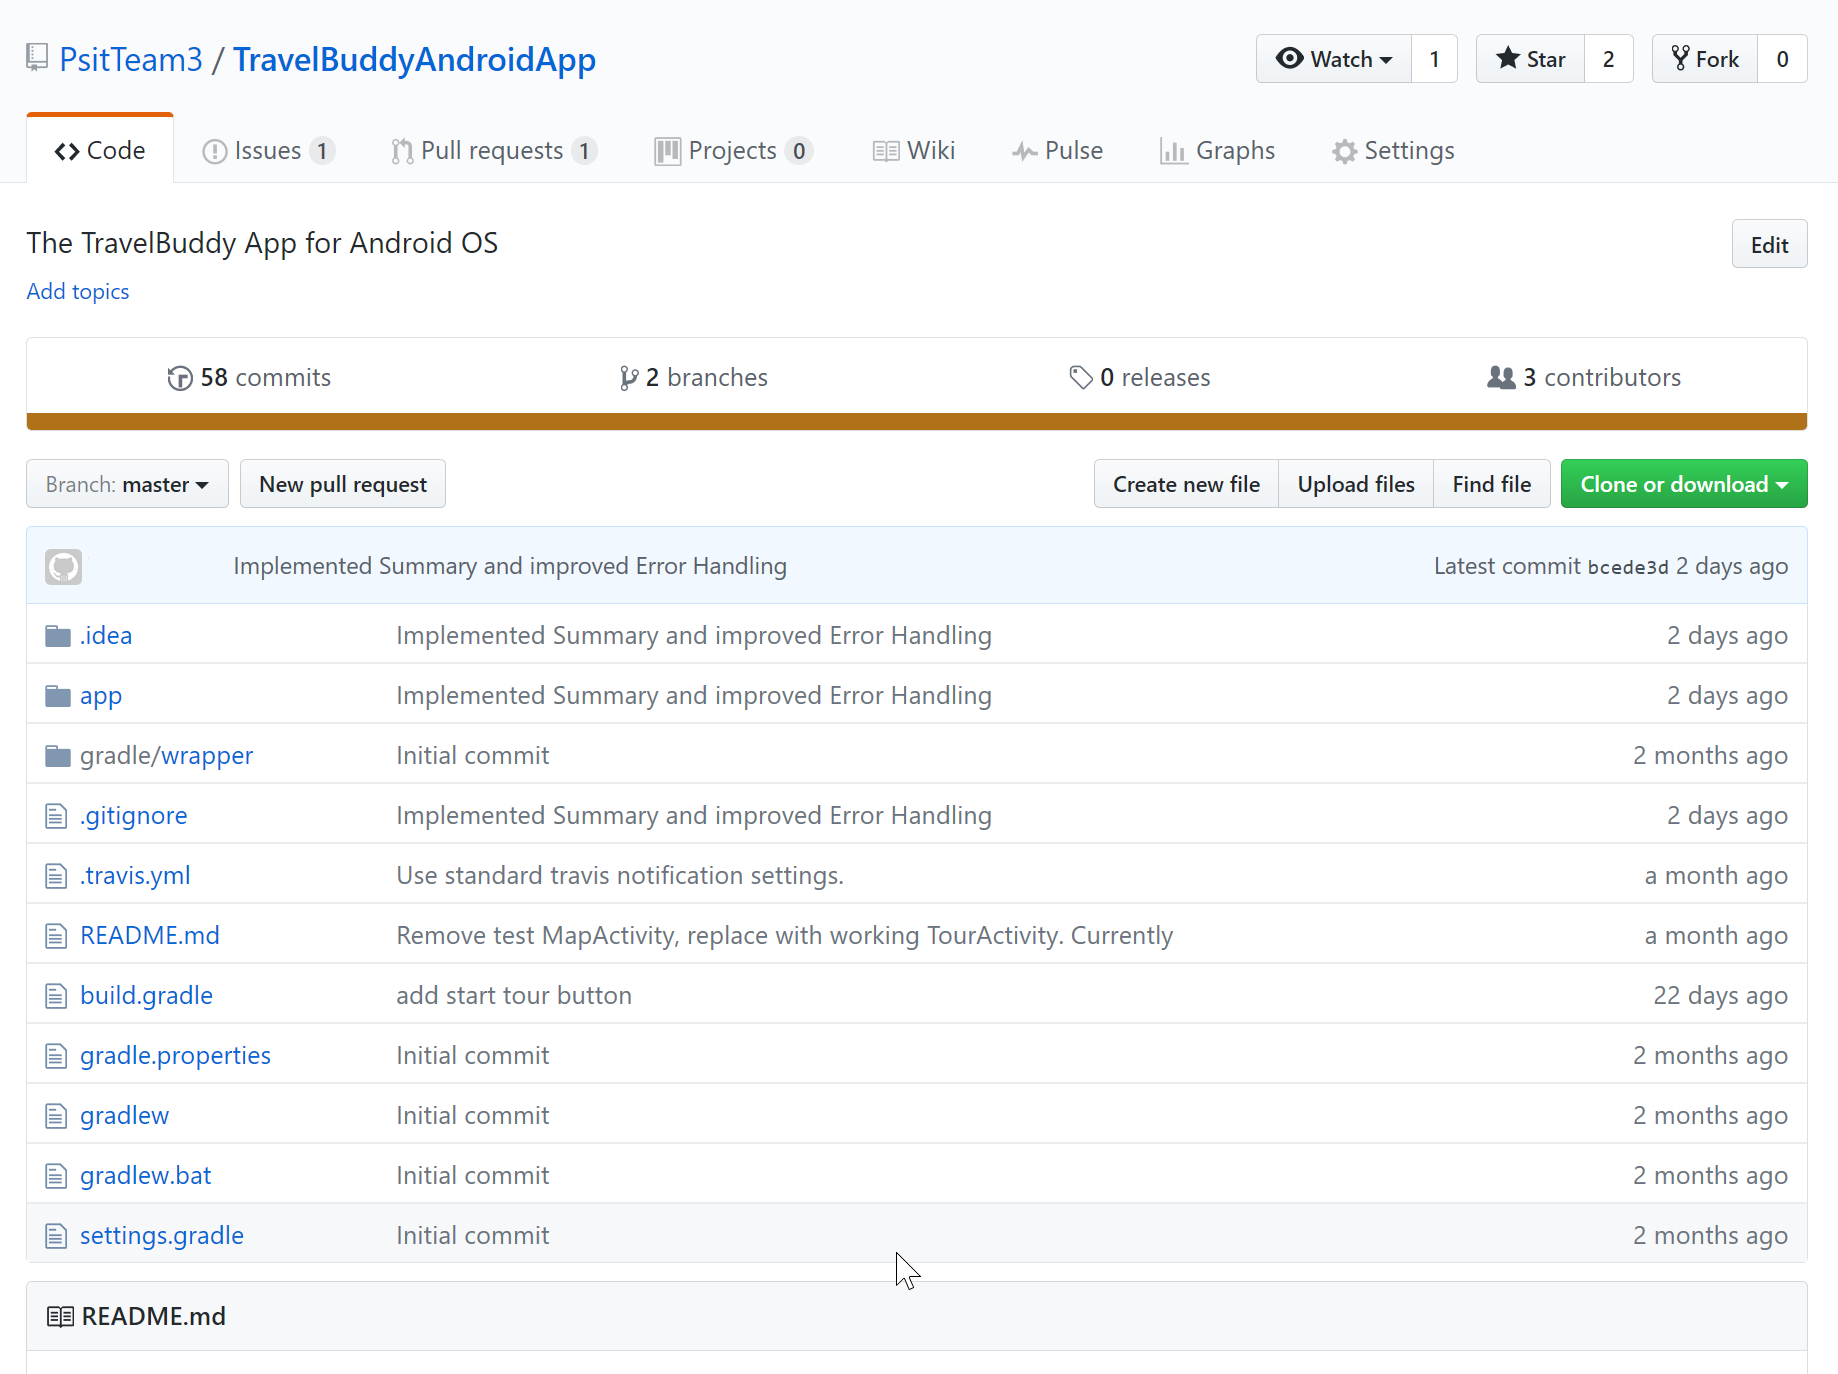
\includegraphics[height=11cm]{Installation/0-0}
  \caption{Übersicht über das Git Projekt}
\end{figure}

\subsubsection{Installation}

\subsubsubsection{Grundinstallation}

Als erstes laden Sie die Installationsdatei von https://developer.android.com/studio/index.html herunter, und starten Sie diese.

\begin{figure}
  \centering
  \begin{minipage}[b]{0.48\textwidth}
    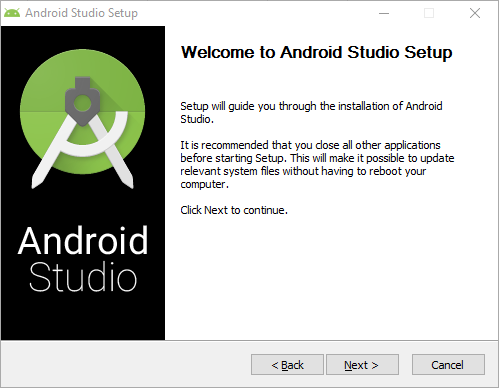
\includegraphics[width=\textwidth]{Installation/1-1}
    \caption{Drücken Sie auf der Willkommensseite auf ``Next''}
  \end{minipage}
  \hfill
  \begin{minipage}[b]{0.48\textwidth}
    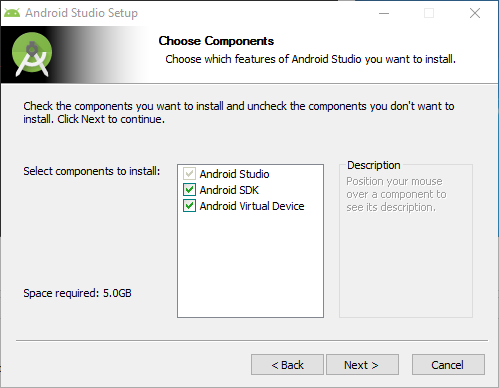
\includegraphics[width=\textwidth]{Installation/1-2}
    \caption{Prüfen Sie ob alle Häckchen gesetzt sind und klicken Sie dann auf ``Next''}
  \end{minipage}
\end{figure}

\begin{figure}
  \centering
  \begin{minipage}[b]{0.48\textwidth}
    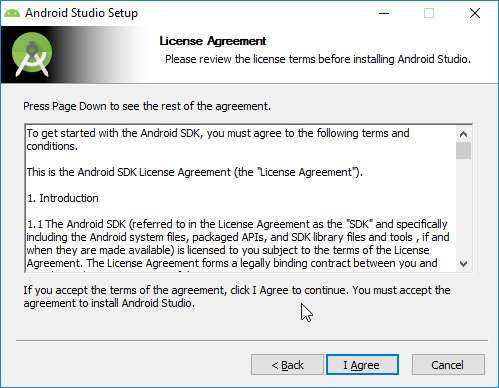
\includegraphics[width=\textwidth]{Installation/1-3}
    \caption{Stimmen Sie der Lizenzvereinbahrung zu, indem Sie auf ``I Agree''}
  \end{minipage}
  \hfill
  \begin{minipage}[b]{0.48\textwidth}
    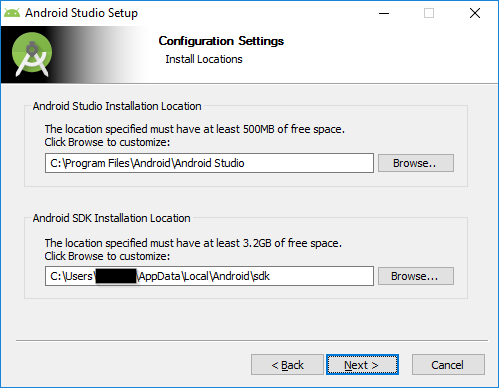
\includegraphics[width=\textwidth]{Installation/1-4}
    \caption{Geben Sie die gewünschten Installationsverzeichnisse an (Im Normalfall sollte nichts angepasst werden müssen) und klicken Sie dann auf ``Next''}
  \end{minipage}
\end{figure}

\begin{figure}
  \centering
  \begin{minipage}[b]{0.48\textwidth}
    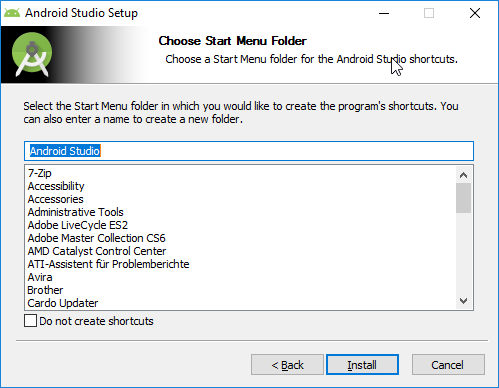
\includegraphics[width=\textwidth]{Installation/1-5}
    \caption{Klicken Sie nun auf ``Install''}
  \end{minipage}
  \hfill
  \begin{minipage}[b]{0.48\textwidth}
    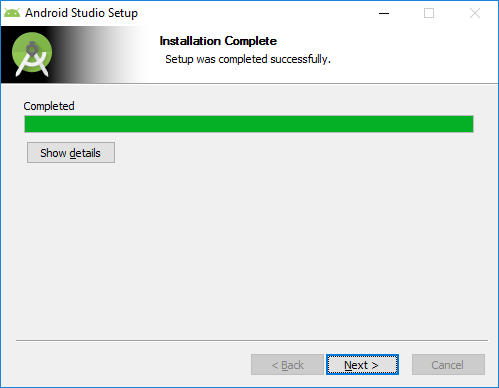
\includegraphics[width=\textwidth]{Installation/1-7}
    \caption{Warten Sie auf das Ende des Installationsvorganges und klicken Sie dann auf ``Next''}
  \end{minipage}
\end{figure}

\begin{figure}
  \centering
  \begin{minipage}[b]{0.48\textwidth}
    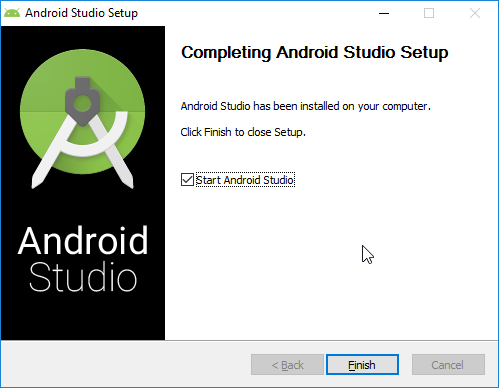
\includegraphics[width=\textwidth]{Installation/1-8}
    \caption{Herzlichen Glückwunsch, Sie haben Android Studio erfolgreich installiert, klicken Sie nun ``Finish''}
  \end{minipage}
  \hfill
  \begin{minipage}[b]{0.48\textwidth}
    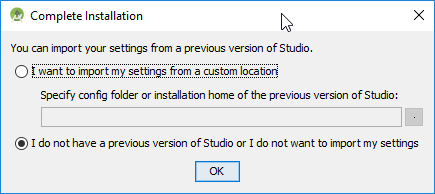
\includegraphics[width=\textwidth]{Installation/1-9}
    \caption{Belassen Sie das Fenster auf ``I do not have a previous\ldots'' und klicken Sie auf ``OK''}
  \end{minipage}
\end{figure}

\begin{figure}
  \centering
  \begin{minipage}[b]{0.48\textwidth}
    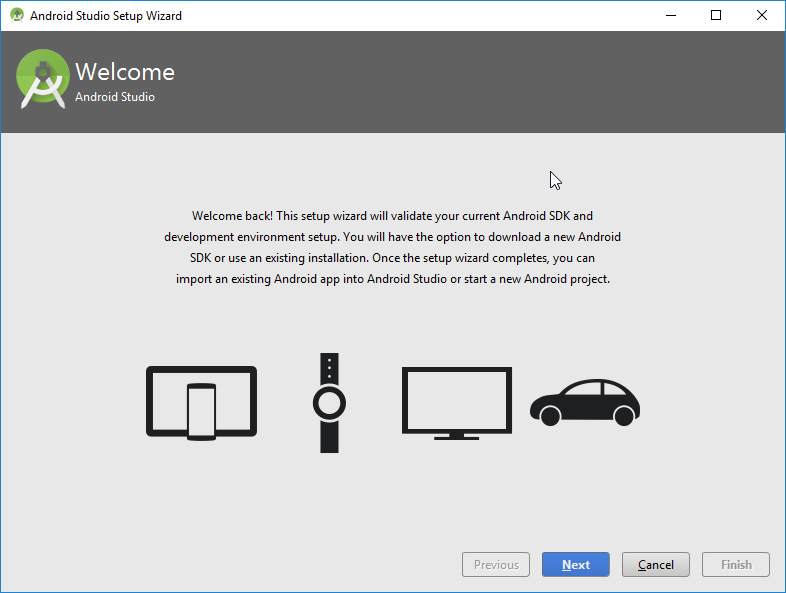
\includegraphics[width=\textwidth]{Installation/1-10}
    \caption{Klicken Sie auf ``Next''}
  \end{minipage}
  \hfill
  \begin{minipage}[b]{0.48\textwidth}
    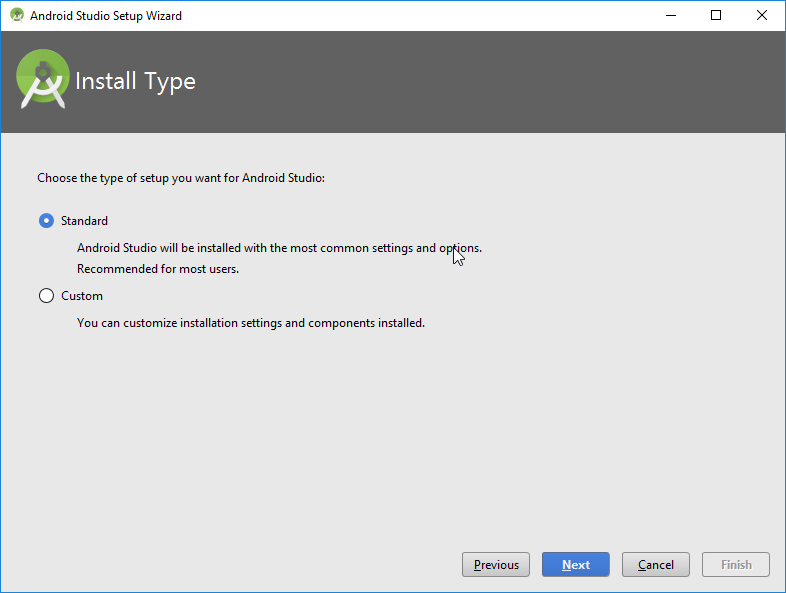
\includegraphics[width=\textwidth]{Installation/1-11}
    \caption{Wählen Sie ``Standard'' und klicken Sie auf ``Next''}
  \end{minipage}
\end{figure}

\begin{figure}
  \centering
  \begin{minipage}[b]{0.48\textwidth}
    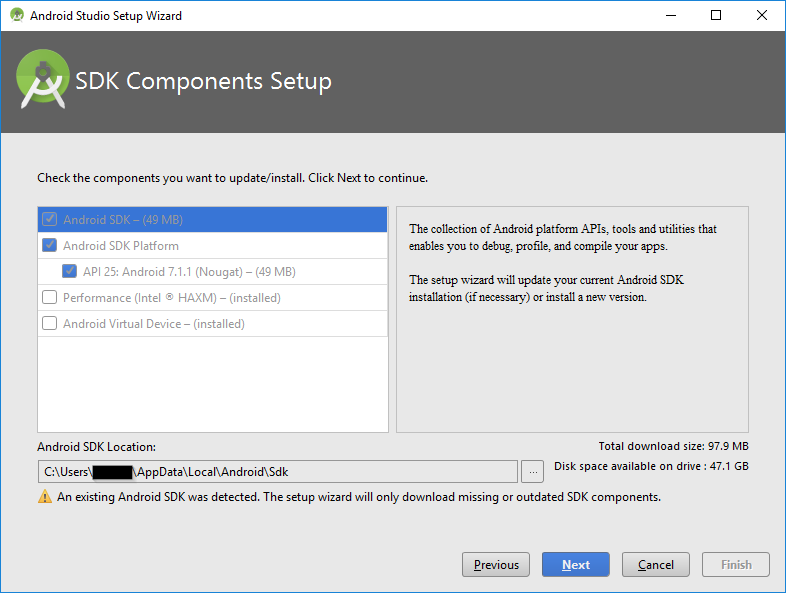
\includegraphics[width=\textwidth]{Installation/1-12}
    \caption{Belassen Sie die Einstellungen und klicken Sie auf ``Next''}
  \end{minipage}
  \hfill
  \begin{minipage}[b]{0.48\textwidth}
    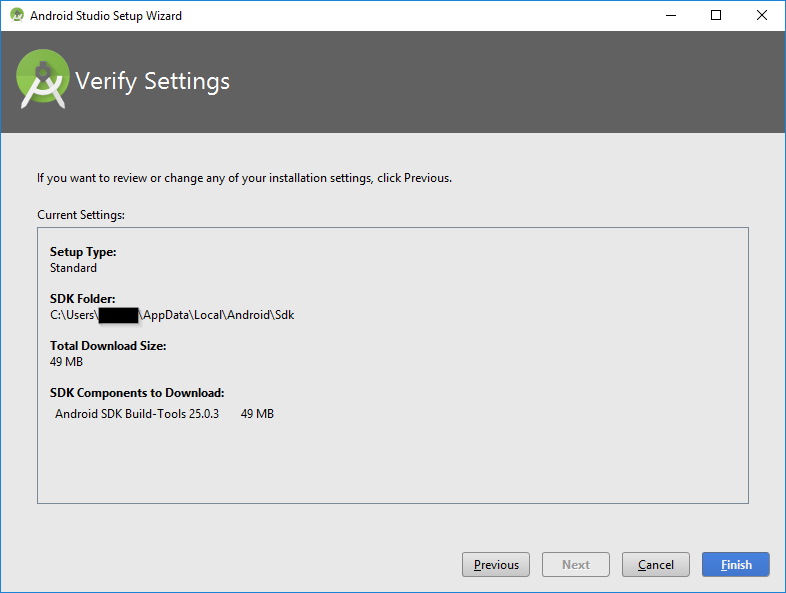
\includegraphics[width=\textwidth]{Installation/1-13}
    \caption{Klicken Sie auf ``Finish''}
  \end{minipage}
\end{figure}

\begin{figure}
  \centering
  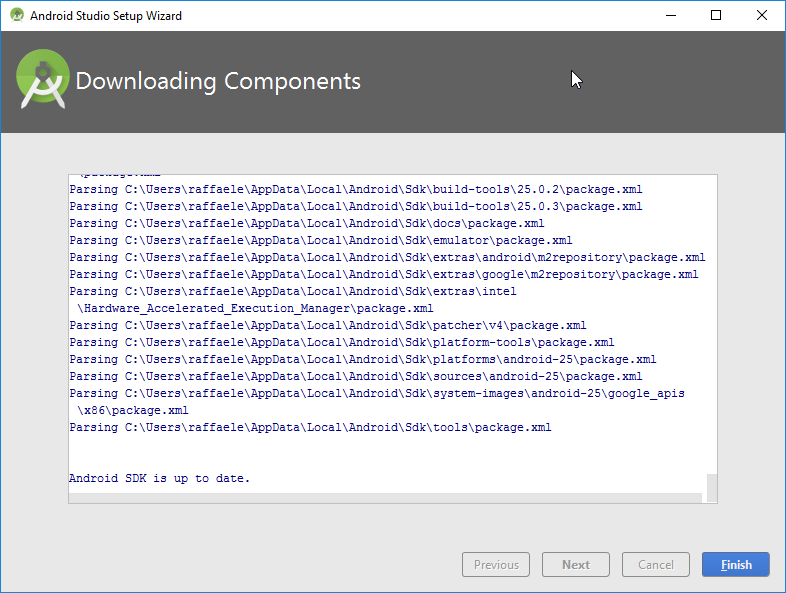
\includegraphics[width=0.48\textwidth]{Installation/1-15}
  \caption{Warten Sie bis der Installationsprozess fertiggestellt ist und klicken Sie auf ``Finish''}
\end{figure}

Herzlichen Glückwunsch, Sie haben nun erfolgreich Android Studio installiert, im nächsten Abschnitt erfahren Sie, wie Sie Android Studio konfigurieren.

\subsubsubsection{Konfiguration}

Da Sie die Installation abgeschlossen haben, müssen Sie noch einige Einstellungen an Android Studio vornehmen, damit Sie an der TravelBuddy Mobile App weiterarbeiten können.

\begin{figure}
  \centering
  \begin{minipage}[b]{0.48\textwidth}
    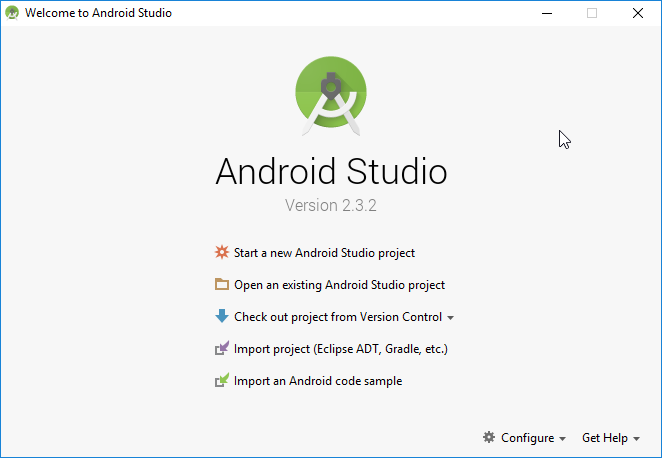
\includegraphics[width=\textwidth]{Installation/2-1}
    \caption{Öffnen Sie nun die lokale Kopie von TravelBuddy indem Sie auf ``Open an existing Android Studio project'' klicken}
  \end{minipage}
  \hfill
  \begin{minipage}[b]{0.48\textwidth}
    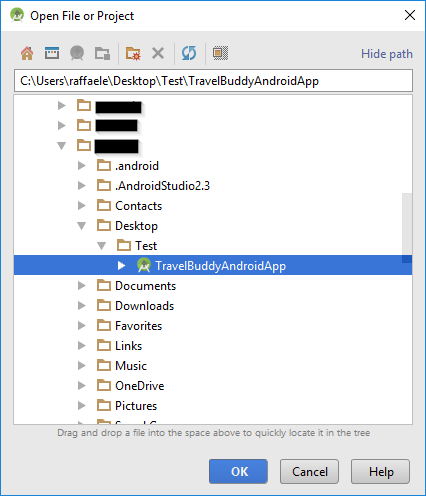
\includegraphics[width=\textwidth]{Installation/2-2}
    \caption{Navigieren Sie zum Pfad ihrer lokalen Kopie von TravelBuddy und klicken Sie auf ``OK''}
  \end{minipage}
\end{figure}

\begin{figure}
  \centering
  \begin{minipage}[b]{0.48\textwidth}
    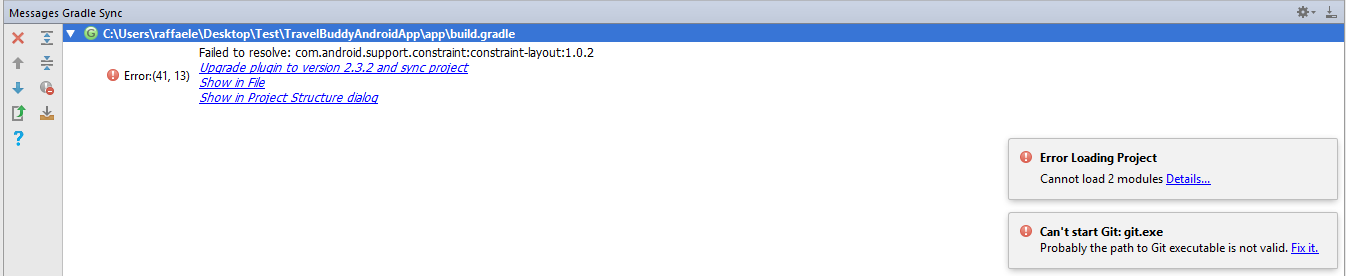
\includegraphics[width=\textwidth]{Installation/2-3}
    \caption{Am unteren Rand sehen Sie nun mehrere Fehlermeldungen, wir starten mit der Meldung ``Can't start Git:git.exe'' klicken Sie hierzu auf ``Fix it'' oder Navigieren Sie zu File-->Settings-->Version Control-->Git}
  \end{minipage}
  \hfill
  \begin{minipage}[b]{0.48\textwidth}
    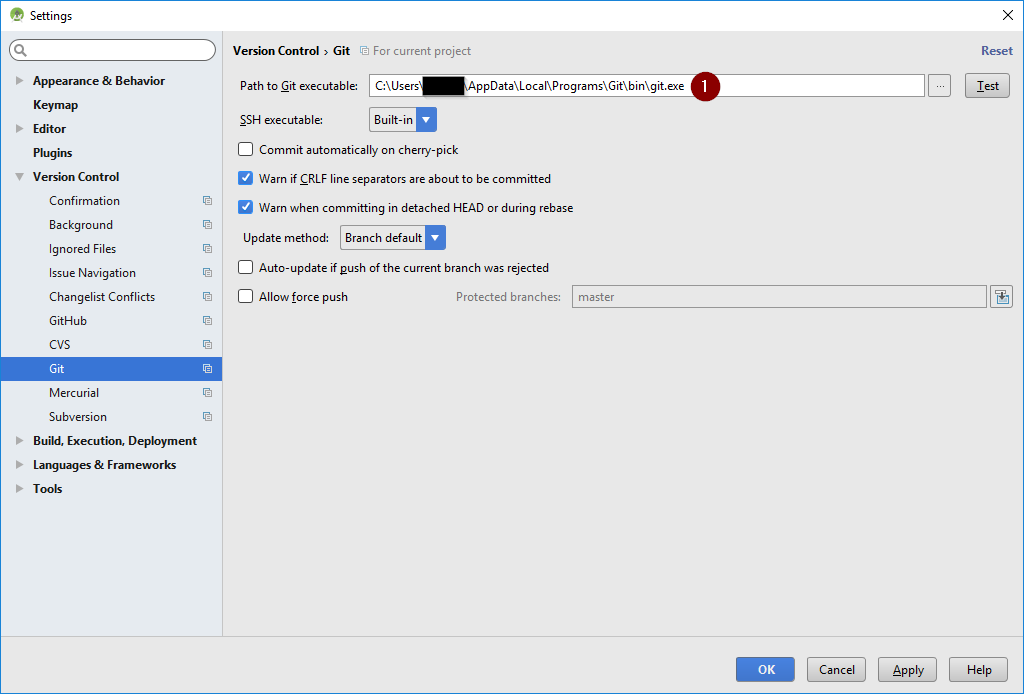
\includegraphics[width=\textwidth]{Installation/2-4}
    \caption{Geben Sie im nun geöffneten Fenster unter ``Path to Git executable''(1) den Pfad zur ausführbaren Datei git.exe Ihrer Git Installation und Bestätigen Sie mit ``OK''}
  \end{minipage}
\end{figure}

\begin{figure}
  \centering
  \begin{minipage}[b]{0.48\textwidth}
    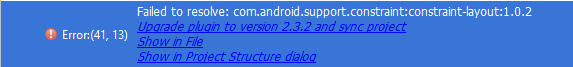
\includegraphics[width=\textwidth]{Installation/2-5}
    \caption{Als nächstes widmen wir uns der oben abgebildeten Fehlermeldung, klicken Sie auf ``Upgrade Plugin \ldots'' und warten Sie bis das Projekt wieder synchronisiert hat.}
  \end{minipage}
  \hfill
  \begin{minipage}[b]{0.48\textwidth}
    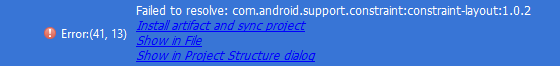
\includegraphics[width=\textwidth]{Installation/2-6}
    \caption{Zu guter letzt widmen wir uns dieser Fehlermeldung, klicken Sie auf ``Install artifact \ldots''}
  \end{minipage}
\end{figure}

\begin{figure}
  \centering
  \begin{minipage}[b]{0.48\textwidth}
    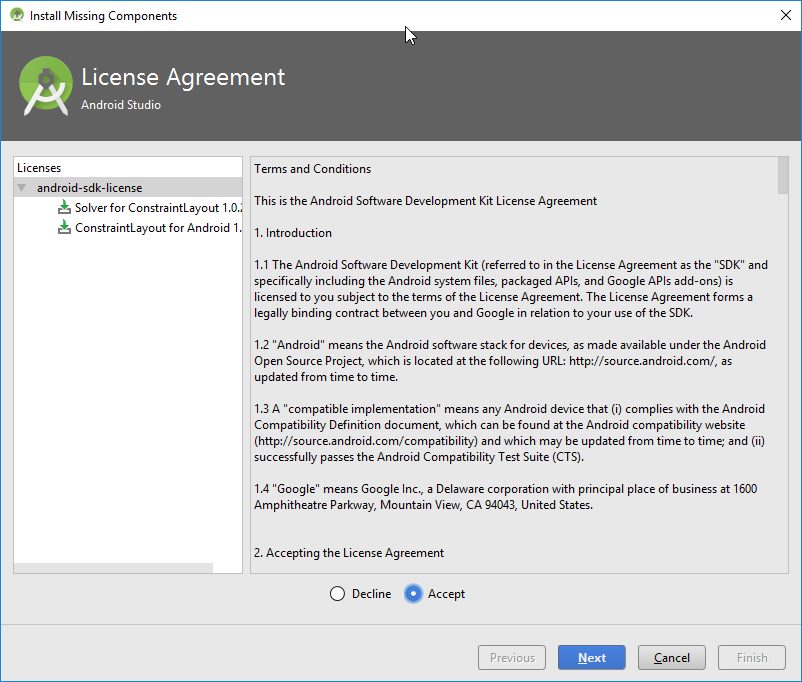
\includegraphics[width=\textwidth]{Installation/2-7}
    \caption{Im neu geöffneten Fenster klicken Sie auf ``Accept'' und anschliessend auf ``Next''}
  \end{minipage}
  \hfill
  \begin{minipage}[b]{0.48\textwidth}
    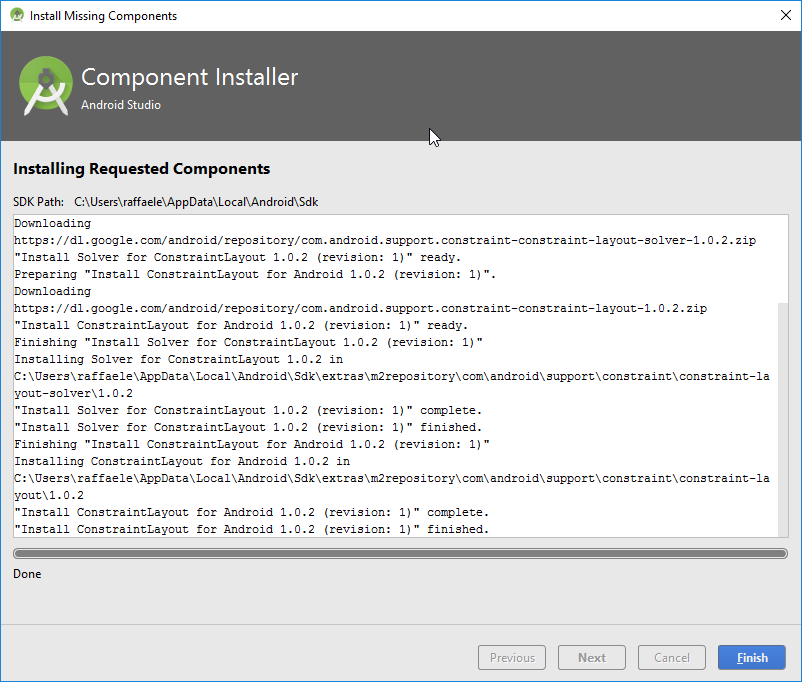
\includegraphics[width=\textwidth]{Installation/2-8}
    \caption{Warten Sie bis der Installationsablauf Fertig ist und klicken Sie dann auf ``Finish''}
  \end{minipage}
\end{figure}

Sie sollten nun in der Lage sein, TravelBuddy zu kompilieren, um ihn ebenfalls zu testen benötigen Sie noch den Android Emulator. Wie Sie diesen Einrichten können, erfahren Sie im nächsten Abschnitt.

\newpage
\subsubsubsection{Emulator einrichten}

Kompilieren Sie nun TravelBuddy, klicken Sie hierzu auf das grüne Dreieck in der oberen Leiste, oder verwenden Sie die Tastenkombination Umschalt + F10.

\begin{figure}
  \centering
  \begin{minipage}[b]{0.48\textwidth}
    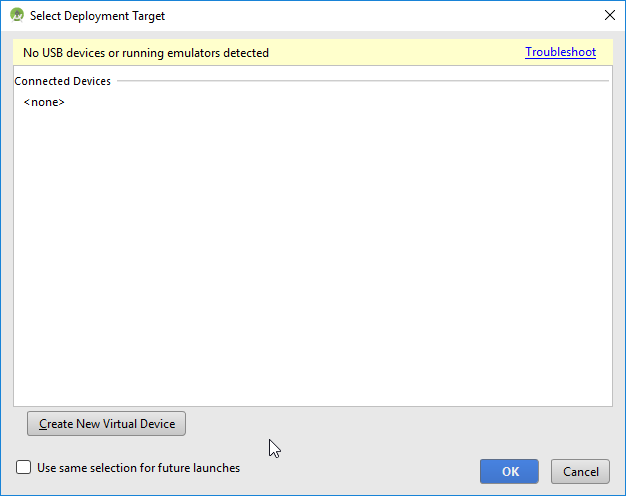
\includegraphics[width=\textwidth]{Installation/3-0}
    \caption{Im nun geöffneten Dialog, klicken Sie auf ``Create New Virtual Device''}
  \end{minipage}
  \hfill
  \begin{minipage}[b]{0.48\textwidth}
    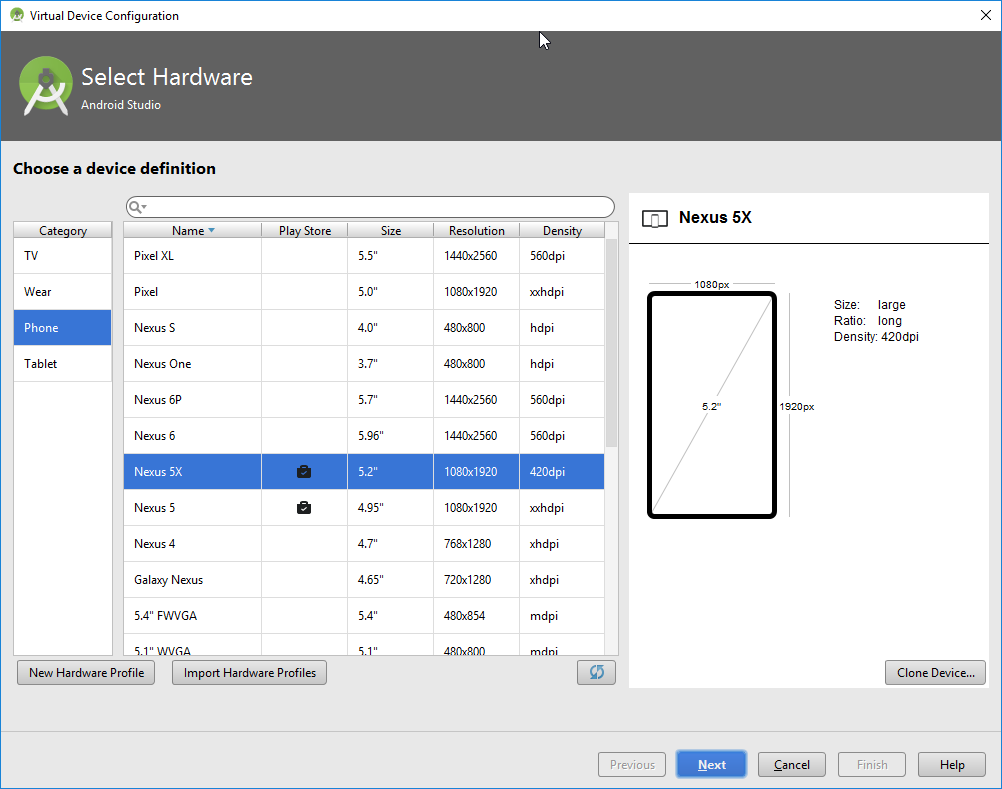
\includegraphics[width=\textwidth]{Installation/3-1}
    \caption{TravelBuddy ist für das Nexus 5X ausgelegt, wählen Sie also dieses und klicken Sie auf ``Next''}
  \end{minipage}
\end{figure}

\begin{figure}
  \centering
  \begin{minipage}[b]{0.48\textwidth}
    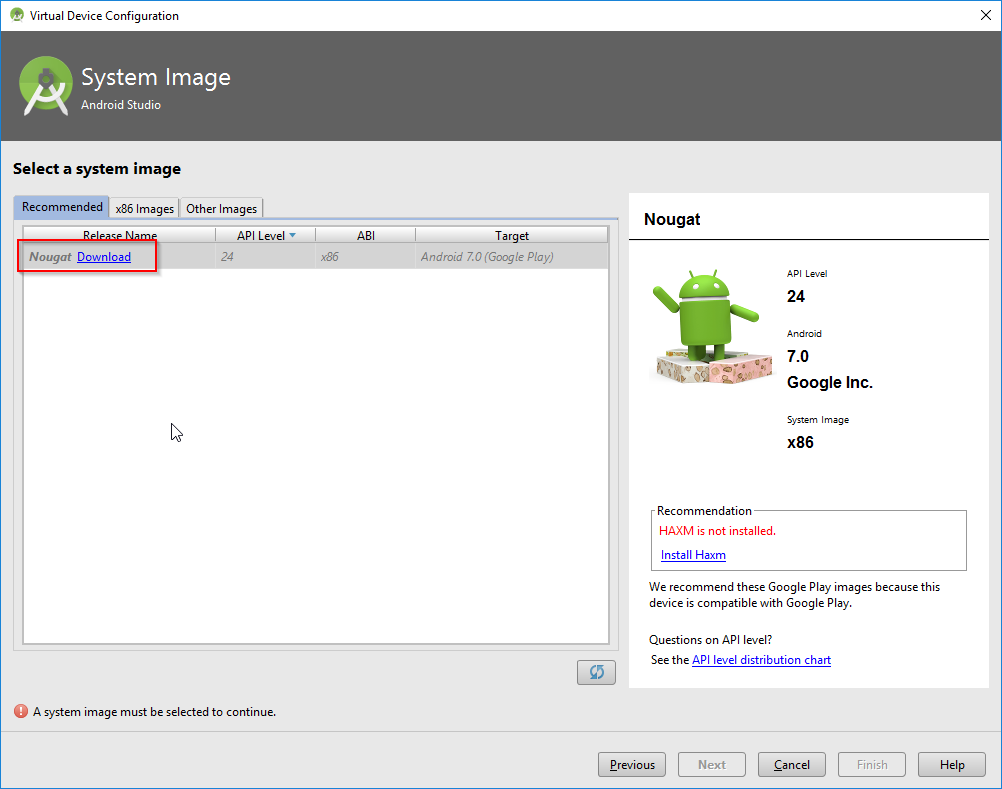
\includegraphics[width=\textwidth]{Installation/3-2}
    \caption{Sie sehen nun eine Liste aller installierbaren Android Betriebssysteme, wählen Sie ``Nougat'' und klicken Sie auf ``Download''}
  \end{minipage}
  \hfill
  \begin{minipage}[b]{0.48\textwidth}
    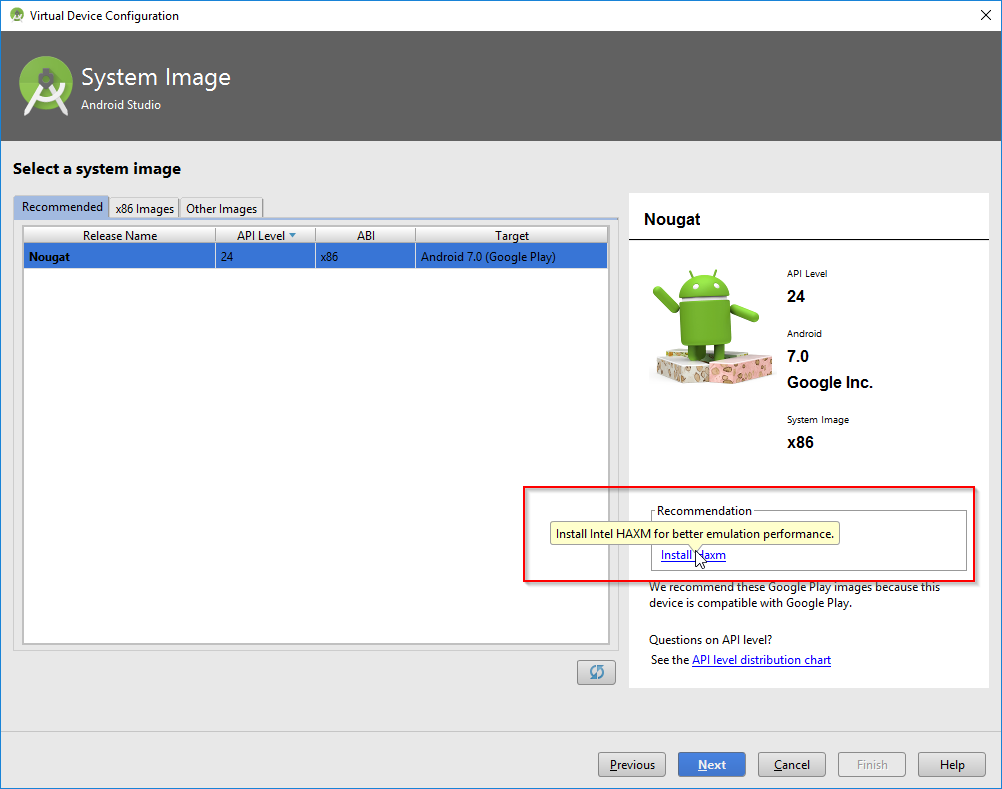
\includegraphics[width=\textwidth]{Installation/3-3}
    \caption{Es fehlt immernoch HAXM, um dies zu installieren klicken Sie auf ``Install HAXM''}
  \end{minipage}
\end{figure}

\begin{figure}
  \centering
  \begin{minipage}[b]{0.48\textwidth}
    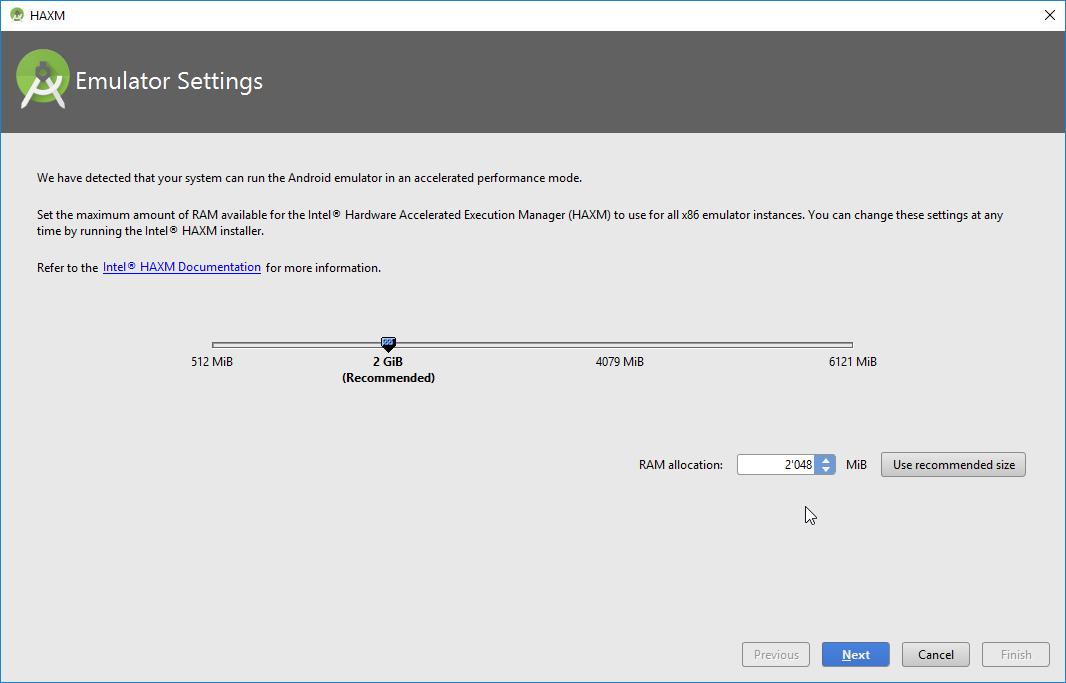
\includegraphics[width=\textwidth]{Installation/3-4}
    \caption{Weisen Sie dem Emulator 2 GiB Arbeitspeicher zu und klicken Sie auf ``Next''}
  \end{minipage}
  \hfill
  \begin{minipage}[b]{0.48\textwidth}
    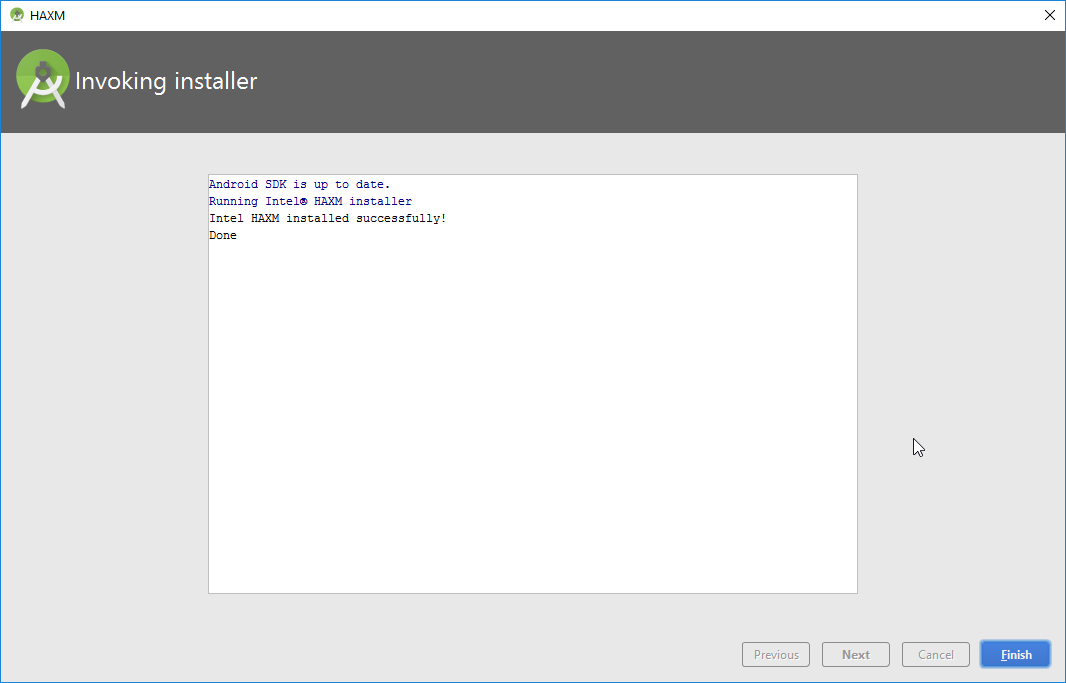
\includegraphics[width=\textwidth]{Installation/3-5}
    \caption{Warten Sie bis der Installationsablauf Fertig ist und klicken Sie dann auf ``Finish''}
  \end{minipage}
\end{figure}

\begin{figure}
  \centering
  \begin{minipage}[b]{0.48\textwidth}
    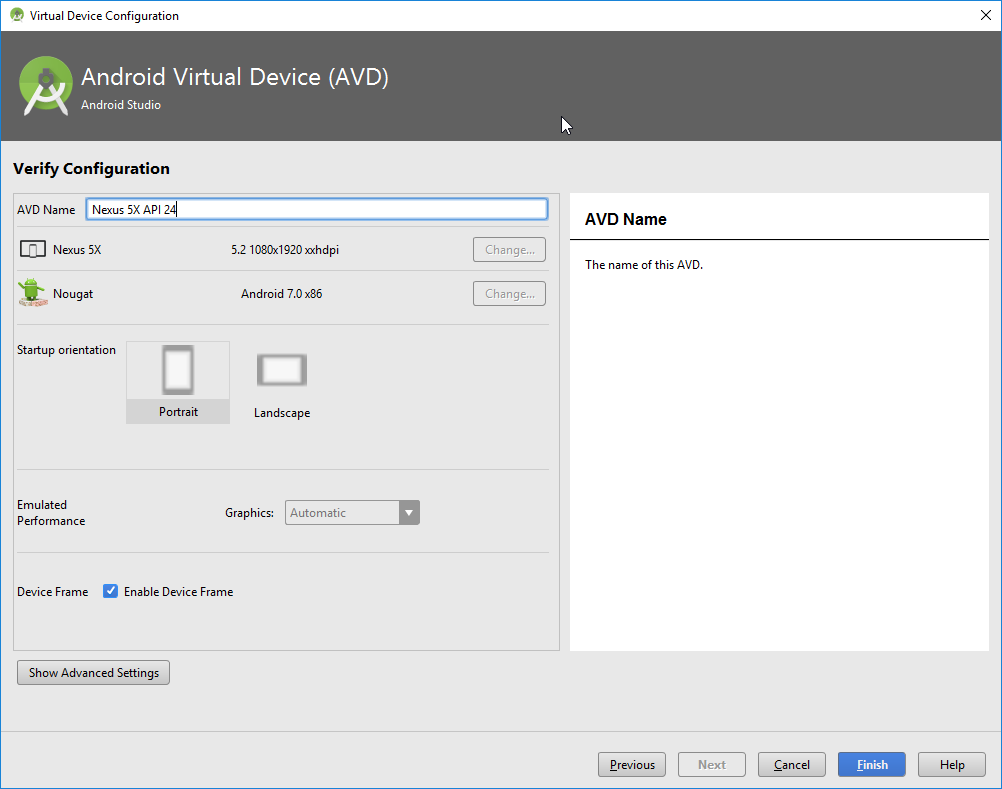
\includegraphics[width=\textwidth]{Installation/3-6}
    \caption{Klicken Sie nun auf ``Finish''}
  \end{minipage}
  \hfill
  \begin{minipage}[b]{0.48\textwidth}
    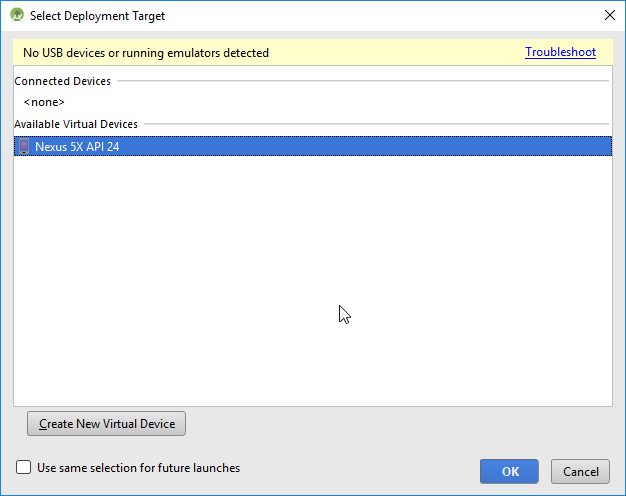
\includegraphics[width=\textwidth]{Installation/3-7}
    \caption{Sie kommen nun zurück in den Dialog aus dem ersten Schritt, mit dem unterschied, dass unter ``Available Virtual Devices'' ein Gerät gelistet sein sollte, wählen Sie dieses aus und klicken Sie auf ``OK''}
  \end{minipage}
\end{figure}

\begin{figure}
  \centering
  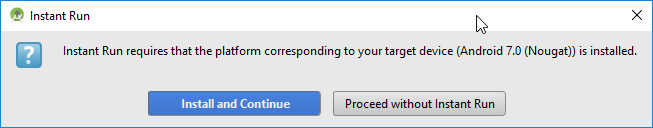
\includegraphics[width=0.48\textwidth]{Installation/3-8}
  \caption{Im nächsten Dialog klicken Sie auf ``Install and Continue''}
\end{figure}

Der Emulator startet nun, wenn er gestartet ist, sollte die kompilierte Version von TravelBuddy automatisch gestartet werden.
\subsubsubsection{Ausführbare Date erstellen}
Nachdem Sie Ihre Weiterentwicklung von TravelBuddy erfolgreich erstellt haben, möchten Sie dieses nun als, auf Android ausführbare Datei (.apk), veröffentlichen.
Der folgende Abschnitt zeigt ihnen wie Sie mit Gradle eine solche Datei generieren können.

\begin{figure}
  \centering
  \begin{minipage}[b]{0.48\textwidth}
    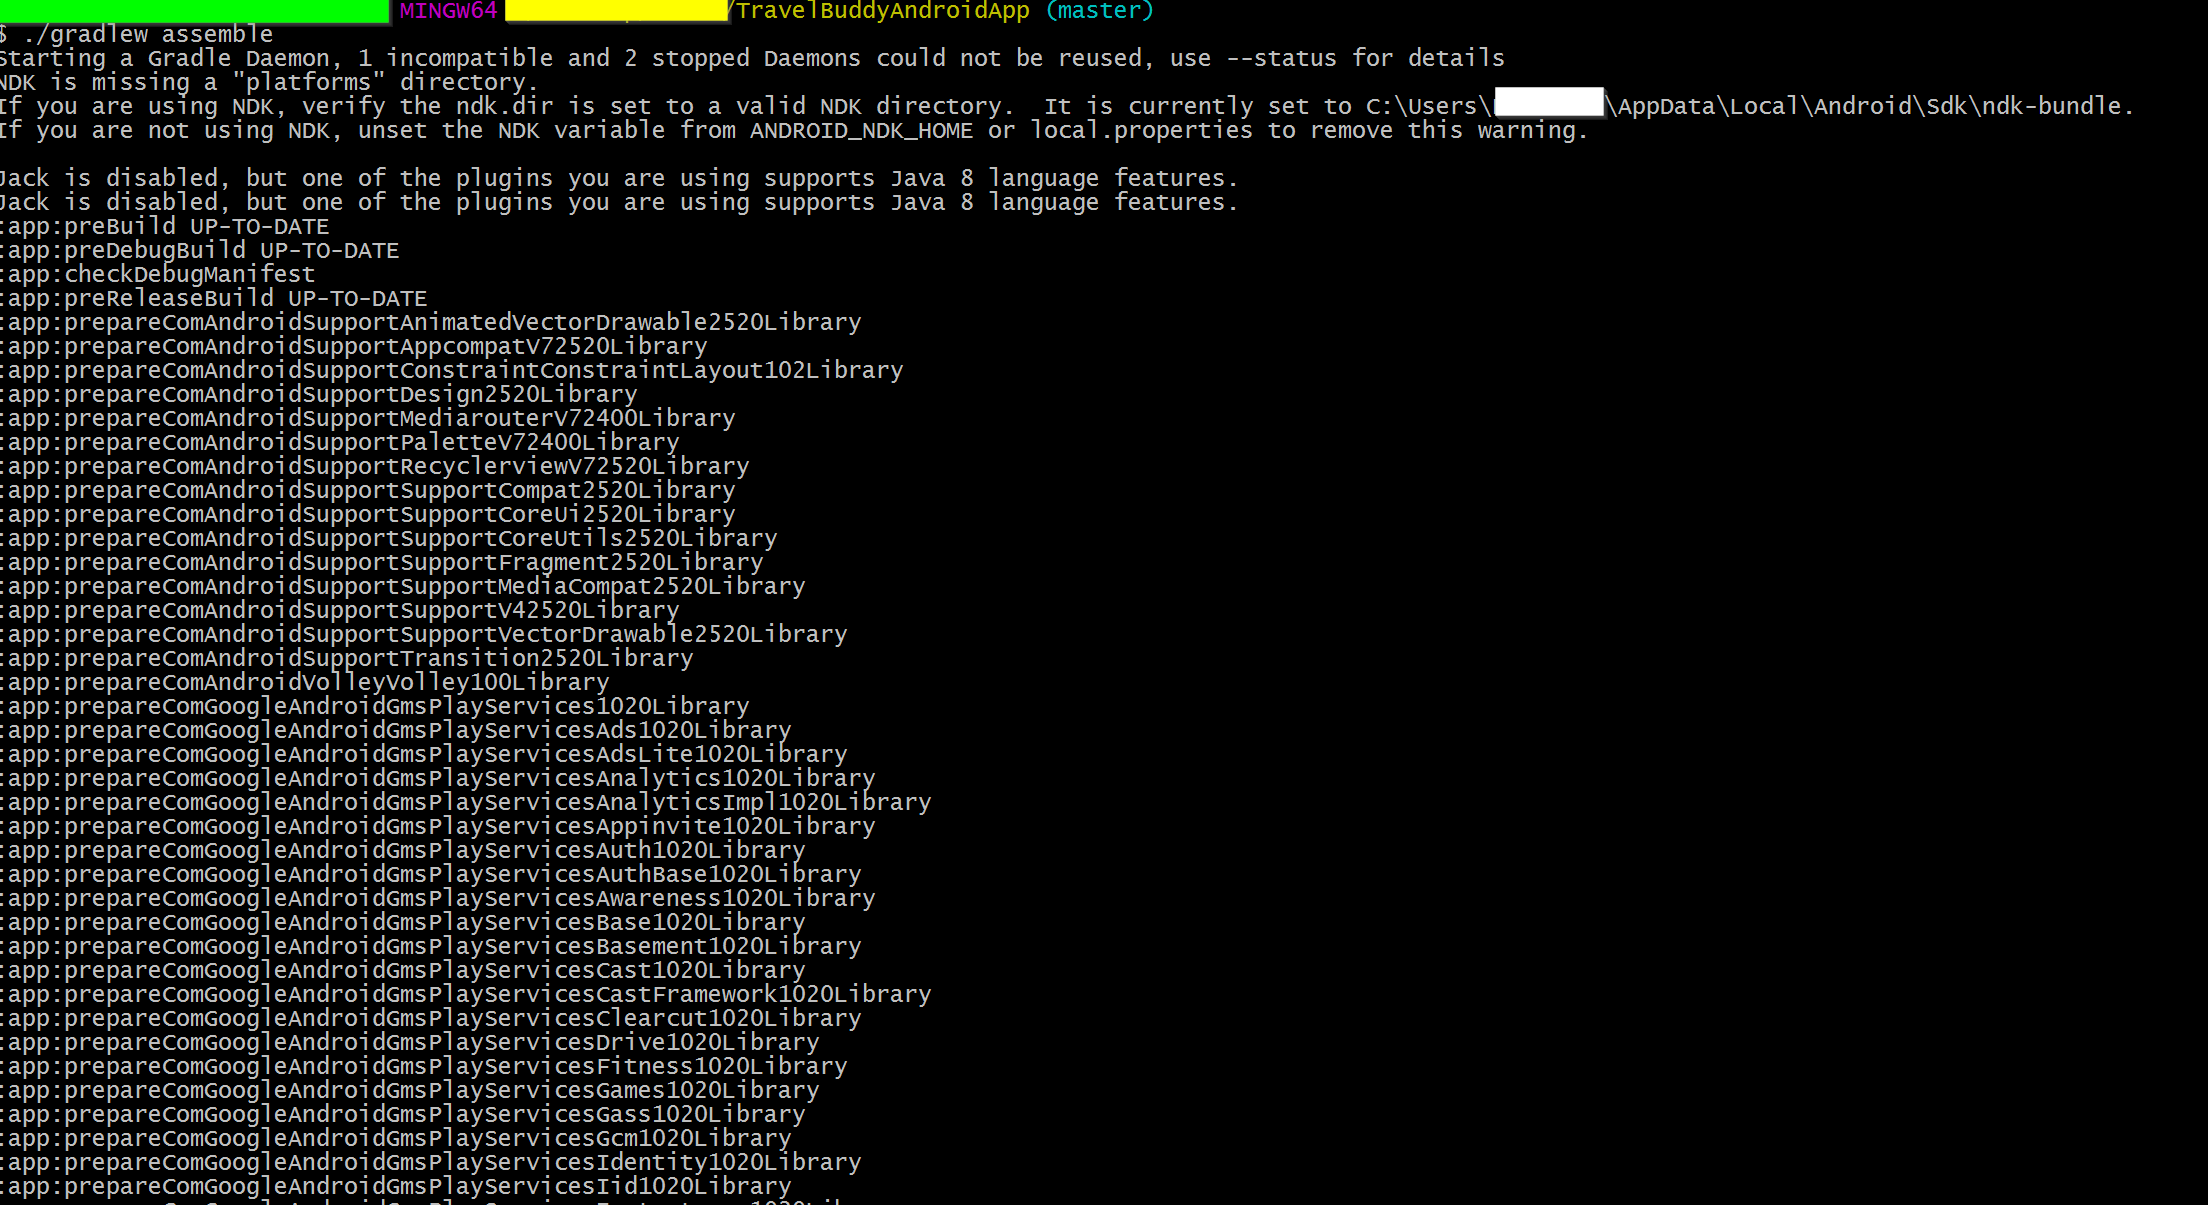
\includegraphics[width=\textwidth]{Installation/4-1}
    \caption{Öffnen Sie die Git Bash Konsole und navigieren Sie in das Hauptverzeichnis des TravelBuddy Projektes. Führen Sie nun den Befehl ``gradlew assemble'' aus und warten Sie.}
  \end{minipage}
  \hfill
  \begin{minipage}[b]{0.48\textwidth}
    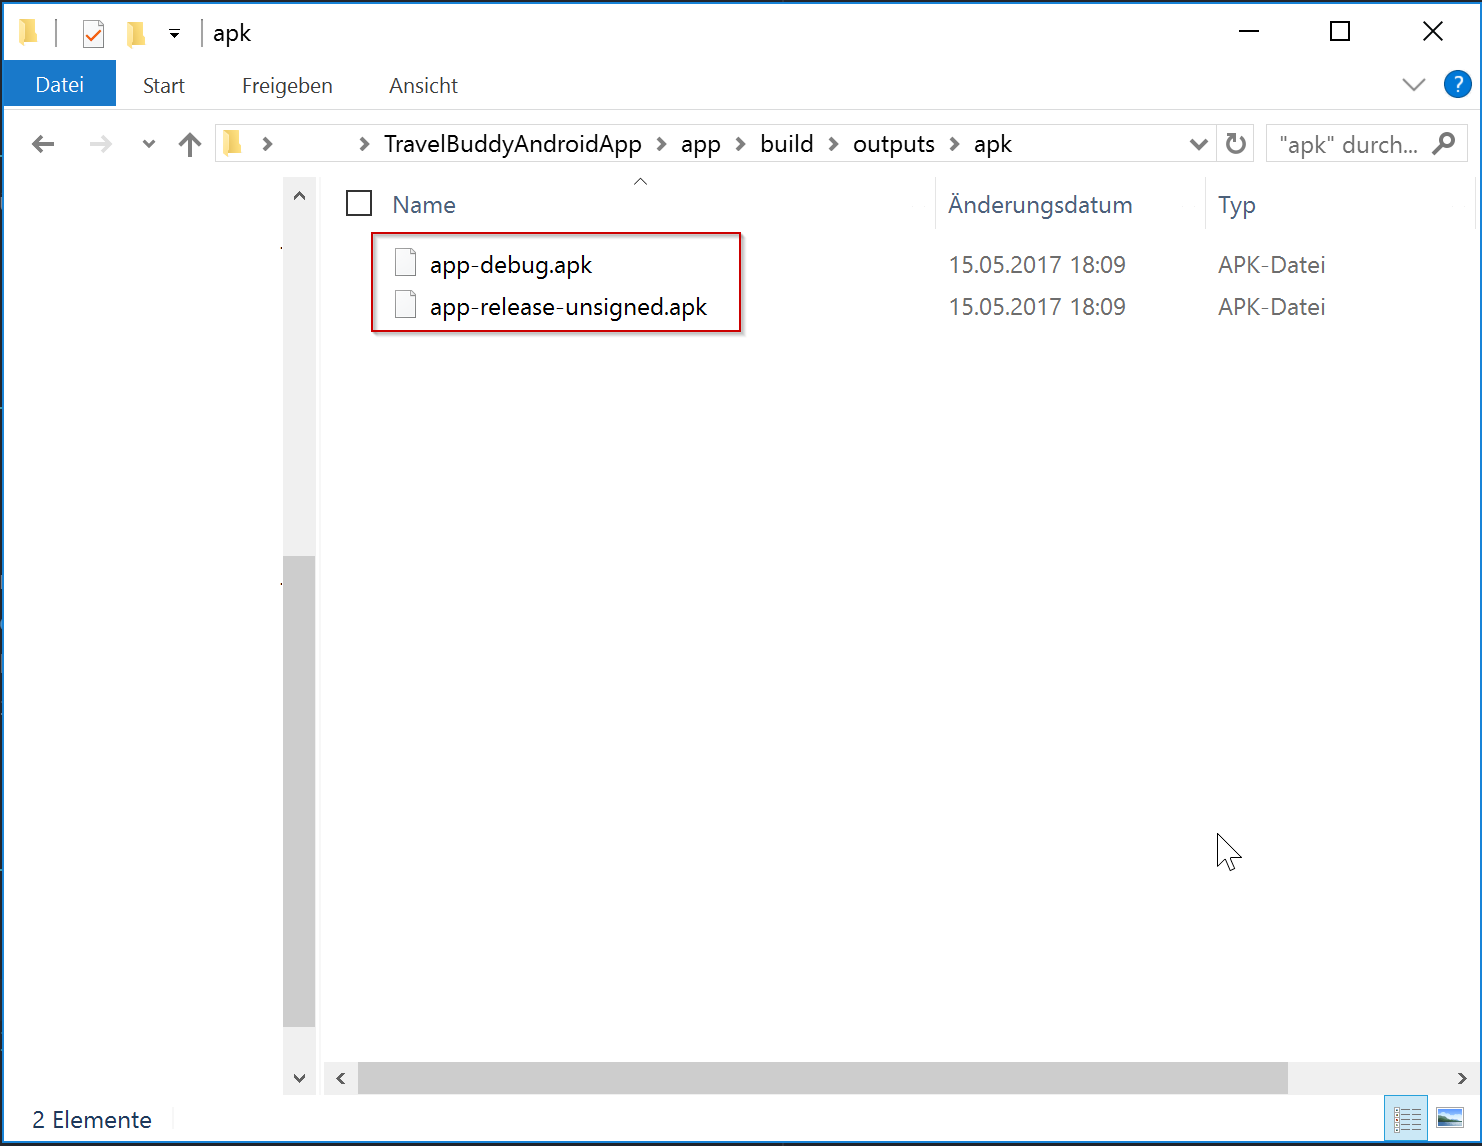
\includegraphics[width=\textwidth]{Installation/4-2}
    \caption{Wenn die Ausführung des Befehles erfolgreich war, finden Sie ihre .apk Datei innerhalb ihrer Kopie des TravelBuddy Projektes im Verzeichnis: TravelBuddyAndroidApp$\backslash$app$\backslash$build$\backslash$outputs$\backslash$apk}
  \end{minipage}
\end{figure}

\subsubsection{Nützliche Links}
  \begin{enumerate}
    \item Git Projekt auf github: https://github.com/PsitTeam3/TravelBuddyAndroidApp
    \item Android Studio Homepage: https://developer.android.com/studio/index.html
    \item API Dokumentation: http://travelbuddy5.azurewebsites.net/swagger/ui/index
  \end{enumerate}
